\documentclass[12pt]{article}
 
\usepackage[margin=1in]{geometry} 
\usepackage{amsmath,amsthm,amssymb}
\usepackage{listings}
\usepackage{tikz}
\usepackage{colortbl}
\usepackage{verbatim}
\usetikzlibrary{arrows, angles, quotes}
\usepackage{framed}

\lstset{basicstyle=\footnotesize}
\usetikzlibrary{calc}

 
\begin{document}
 
\title{Contradiction\\
    \large CS101A Problem Solving I}
\author{Harry Coleman}
\date{October 8, 2019}

\maketitle

\section*{Problem 4}
\fbox{
    \parbox{\textwidth}{
        Show that there are no positive integer solutions to the Diophantine equation $x^2 - y^2 = 1$.
    }
}
\\

\begin{align*}
    x^2 - y^2 &= 1 \\
    (x+y)(x-y) & = 1
\end{align*}

We will first assume that there exists some positive integer solution to the equation. Since we are looking for positive integer solutions for $x$ and $y$, and the integers are closed under addition, subtraction, and multiplication
\[\begin{cases}
    x+y = 1 \\
    x-y = 1
\end{cases}\]
\begin{align*}
    2x &= 2 \\
    x &= 1 \\
    1 + y &= 1 \\
    y & = 0 \\
\end{align*}

This contradicts our assumption since $y=0$ is not a positive integer solution. Therefore, there are no positive integer solutions to the Diophantine equation $x^2 - y^2 = 1$.


\newpage
\section*{Problem 5}
\fbox{
    \parbox{\textwidth}{
        Show that the equation
        \[b^2 + b + 1 = a^2\]
        has no positive integer solutions.
    }
}
\\

We will assume that there is some positive integer solution for $a$ and $b$. Since $b$ is postive, we know that
\begin{gather*}
    b^2 < b^2 + b + 1 < b^2 + 2b + 1 \\
    b^2 < a^2 < (b+1)^2 \\
    b < a < b+1
\end{gather*}

So $a$ is some integer between two consecutive integers. This, however, is not possible and therefore a contradiction, so our assumption cannot be true. Therefore
\[b^2 + b + 1 = a^2\]
has no positive integer solutions.


\newpage
\section*{Problem 6}
\fbox{
    \parbox{\textwidth}{
        Prove that there is no polynomial $P(x) = a_nx^n + a_{n-1}x^{n-1} + ... + a_0$ with integer coefficients and of degree at least 1 with the property that P(0), P(1), P(2),... are all prime numbers.
    }
}
\\

First, we will assume that $\forall (x \in \{0, 1, 2,...\})[P(x) \text{ is prime}]$. So
\begin{align*}
    P(0) &= a_n(0)^n + a_{n-1}(0)^{n-1} + ... + a_0 \\
         &= 0 + 0 + ... + a_0 \\
         &= a_0
\end{align*}

Therefore $a_0$ is some prime number. Because every term has integer coefficients, we also know that
\[P(ka_0) = a_n(ka_0))^n + a_{n-1}(ka_0))^{n-1} + ... + a_0\]
where $k \in \mathbb{N}$. So $P(ka_0)$ is some integer divisible by $a_0$. Since $P(ka_0)$ is a prime number, and the only prime number divisible by $a_0$ is $a_0$,
\[\forall(k \in \mathbb{N})[P(ka_0)=a_0]\]

The only time $P(x)=a_0$ is when all the terms preceding $a_0$ sum to 0. So if we define
\begin{align*}
    P_2(x) &= a_nx^n + a_{n-1}x^{n-1} + ... + a_1x^1 \\
    P_2(x) &= P(x) - a_0
\end{align*}

then
\[\forall(k \in \mathbb{N})[P_2(ka_0) = 0]\]
meaning that 
\[\forall(k \in \mathbb{N})[ka_0 \text{ is a root of } P_2(x)]\]

We know that $P(x)$ is a polynomial of degree $n>1$. So $P_2(x)$ is also a polynomial of degree $n>1$ since $P_2(x)$ includes the highest degree term of $P(x)$. This means that $P_2(x)$ can have at most $n$ real roots. Because we can construct a set
\[M = \{ka_0 \mid k \in \{1, 2, 3,..., n, n+1\}\}\]
which is a set of $n+1$ multiples of $a_0$, 
\begin{align*}
    &\exists (m \in M)[m \text{ is not a root of } P_2(x)] \\
    &\exists (m \in M)[P_2(m) \ne 0] \\
    &\exists (k \in \mathbb{N})[P_2(ka_0) \ne 0]
\end{align*}

So we have 
\[\forall(k \in \mathbb{N})[P_2(ka_0) = 0]\]
\[\exists (k \in \mathbb{N})[P_2(ka_0) \ne 0]\]


\newpage
\section*{Problem 7}
\fbox{
    \parbox{\textwidth}{
        Show that there does not exist a function $f : \mathbb{Z} \rightarrow \{1,2,3\}$ satisfying $f(x) \ne f(y)$ for all $x,y \in \mathbb{Z}$ such that $\left|x - y\right| \in \{2,3,5\}$.
    }
}
\\

We will look at an arbitrary interval on the set of integers $[n, n+7]$ and (assuming that we can) construct a portion of a mapping from the integers to 3 distinct values satisfying $f(x) \ne f(y)$ for all $x,y \in \mathbb{Z}$ such that $\left|x - y\right| \in \{2,3,5\}$. Instead of $\{1,2,3\}$ we will use $\{A,B,C\}$. 

We will use the below table to show our mapping as we construct it. The top row shows the position of sequential integers. The highlighted row will show our mapping. And the bottom three rows show the possible values of \{A,B,C\} that can go in that position, based on the conditions for $f$. It should 


\begin{center}
    \begin{tabular}{|c|c|c|c|c|c|c|c|}
        \hline
        $n+0$ & $n+1$ & $n+2$ & $n+3$ & $n+4$ & $n+5$ & $n+6$ & $n+7$ \\
        \hline
        \rowcolor[RGB]{200, 200, 200}
         & & & & & & & \\
        \hline
        A & A & A & A & A & A & A & A \\
        \hline
        B & B & B & B & B & B & B & B \\
        \hline
        C & C & C & C & C & C & C & C \\
        \hline
    \end{tabular}
\end{center}

We will first assign $A$ to the first position. New values will be highlighted, as well as the values that become restricted by the new value.
\begin{center}
    \begin{tabular}{|c|c|c|c|c|c|c|c|}
        \hline
        $n+0$ & $n+1$ & $n+2$ & $n+3$ & $n+4$ & $n+5$ & $n+6$ & $n+7$ \\
        \hline
        \rowcolor[RGB]{200, 200, 200}
        \cellcolor{gray!70}A & & & & & & & \\
        \hline
        A & A & \cellcolor{gray!15} & \cellcolor{gray!15} & A & \cellcolor{gray!15} & A & A \\
        \hline
        B & B & B & B & B & B & B & B \\
        \hline
        C & C & C & C & C & C & C & C \\
        \hline
    \end{tabular}
\end{center}

We can see that the positions 2, 3, and 5 units away from $n$ cannot be assigned a value of $A$, so we will pick something other than $A$ for $n+2$.
\begin{center}
    \begin{tabular}{|c|c|c|c|c|c|c|c|}
        \hline
        $n+0$ & $n+1$ & $n+2$ & $n+3$ & $n+4$ & $n+5$ & $n+6$ & $n+7$ \\
        \hline
        \rowcolor[RGB]{200, 200, 200}
        A & &\cellcolor{gray!70} B & & & & & \\
        \hline
        A & A &  &  & A &  & A & A \\
        \hline
        \cellcolor{gray!15} & B & B & B & \cellcolor{gray!15} & \cellcolor{gray!15} & B & \cellcolor{gray!15} \\
        \hline
        C & C & C & C & C & C & C & C \\
        \hline
    \end{tabular}
\end{center}

We now see in the $n+5$ position that there is only one possible value. We will now continue to fill out this table, restricting ourselves to putting in values only when there is one possibility.
\begin{center}
    \begin{tabular}{|c|c|c|c|c|c|c|c|}
        \hline
        $n+0$ & $n+1$ & $n+2$ & $n+3$ & $n+4$ & $n+5$ & $n+6$ & $n+7$ \\
        \hline
        \rowcolor[RGB]{200, 200, 200}
        A & & B & & &\cellcolor{gray!70} C & & \\
        \hline
        A & A &  &  & A &  & A & A \\
        \hline
         & B & B & B &  &  & B &  \\
        \hline
        \cellcolor{gray!15} & C & \cellcolor{gray!15} & \cellcolor{gray!15} & C & C & C & \cellcolor{gray!15} \\
        \hline
    \end{tabular}
\end{center}

\begin{center}
    \begin{tabular}{|c|c|c|c|c|c|c|c|}
        \hline
        $n+0$ & $n+1$ & $n+2$ & $n+3$ & $n+4$ & $n+5$ & $n+6$ & $n+7$ \\
        \hline
        \rowcolor[RGB]{200, 200, 200}
        A & & B & & & C & &\cellcolor{gray!70} A \\
        \hline
        A & A & \cellcolor{gray!15} &  & \cellcolor{gray!15} & \cellcolor{gray!15} & A & A \\
        \hline
         & B & B & B &  &  & B &  \\
        \hline
         & C &  &  & C & C & C &  \\
        \hline
    \end{tabular}
\end{center}

\begin{center}
    \begin{tabular}{|c|c|c|c|c|c|c|c|}
        \hline
        $n+0$ & $n+1$ & $n+2$ & $n+3$ & $n+4$ & $n+5$ & $n+6$ & $n+7$ \\
        \hline
        \rowcolor[RGB]{200, 200, 200}
        A & & B &\cellcolor{gray!70} B & & C & & A \\
        \hline
        A & A &  &  &  &  & A & A \\
        \hline
         & \cellcolor{gray!15} & B & B &  & \cellcolor{gray!15} & \cellcolor{gray!15} &  \\
        \hline
         & C &  &  & C & C & C &  \\
        \hline
    \end{tabular}
\end{center}

\begin{center}
    \begin{tabular}{|c|c|c|c|c|c|c|c|}
        \hline
        $n+0$ & $n+1$ & $n+2$ & $n+3$ & $n+4$ & $n+5$ & $n+6$ & $n+7$ \\
        \hline
        \rowcolor[RGB]{200, 200, 200}
        A & & B & B &\cellcolor{gray!70} C & C & & A \\
        \hline
        A & A &  &  &  &  & A & A \\
        \hline
         &  & B & B &  &  &  &  \\
        \hline
         & \cellcolor{gray!15} & \cellcolor{gray!15} &  & C & C & \cellcolor{gray!15} & \cellcolor{gray!15} \\
        \hline
    \end{tabular}
\end{center}

\begin{center}
    \begin{tabular}{|c|c|c|c|c|c|c|c|}
        \hline
        $n+0$ & $n+1$ & $n+2$ & $n+3$ & $n+4$ & $n+5$ & $n+6$ & $n+7$ \\
        \hline
        \rowcolor[RGB]{200, 200, 200}
        A &\cellcolor{gray!70} A & B & B & C & C & & A \\
        \hline
        A & A &  & \cellcolor{gray!15} & \cellcolor{gray!15} &  & \cellcolor{gray!15} & A \\
        \hline
         &  & B & B &  &  &  &  \\
        \hline
         &  &  &  & C & C &  &  \\
        \hline
    \end{tabular}
\end{center}

We now see that $n+6$ cannot be any value of $\{A,B,C\}$. This contradicts our assumption that a mapping was possible. Therefore, there cannot exist a function $f : \mathbb{Z} \rightarrow \{A,B,C\}$ satisfying $f(x) \ne f(y)$ for all $x,y \in \mathbb{Z}$ such that $\left|x - y\right| \in \{2,3,5\}$. For which we can just as easily specify $\{A,B,C\} = \{1,2,3\}$.


\newpage
\section*{Problem 8}
\fbox{
    \parbox{\textwidth}{
        Every point of the three-dimensional space is colored red, green, or blue. Prove that one of the colors attains all distances, meaning that any positive real number represents the distance between two points of this color.
    }
}
\\

We will use $A$, $B$, and $C$ as our 3 colors, each is interchangeable for any one color different from the other two. First, we will assume that it is possible for our three-dimensional space to be colored in the described way. We will define a function $S(x)$ where $x \in \{A, B, C\}$ which returns the set of all attainable distances of the given color $x$. Because no one color attains all distances, we can say

\[\forall(x \in \{A, B, C\})[\exists (d_x \in \mathbb{R}_{>0}) \notin S(x)]\]
or
\begin{align*}
    \exists (d_A \in \mathbb{R}_{>0}) \notin S(A) \\
    \exists (d_B \in \mathbb{R}_{>0}) \notin S(B) \\
    \exists (d_C \in \mathbb{R}_{>0}) \notin S(C)
\end{align*}

Because $A$, $B$, and $C$ are interchangeable, we'll say that

\[d_A \geq d_B \geq d_C\]

Around some point in our space that is colored $A$, we know that there must be a sphere of radius $d_A$ around that point on which no point is colored $A$. Since if there was a point on the sphere colored $A$, the distance between that $A$ point and the center $A$ point would be $d_A$, but $d_A \notin S(A)$. So all the points on the sphere are $B$ or $C$.

\begin{center}
    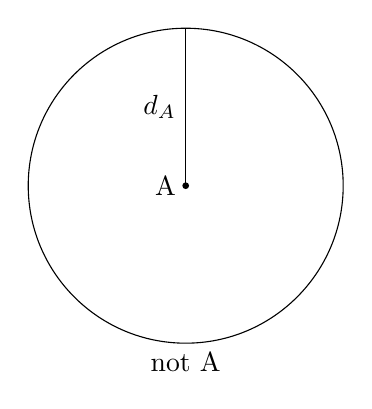
\begin{tikzpicture}
        \coordinate (A) at (0,0);
        \coordinate (Ar) at (0,2);
        \coordinate (Ac) at (0, -2);
        
        \filldraw[black] (A) circle (1pt) node[anchor=east] {A};
        \draw (A) -- node[anchor=east]{$d_A$} ++ (Ar);
        \draw[black] (A) circle (2cm);
        \draw (Ac) node[anchor=north] {not A};
        
    \end{tikzpicture}
\end{center}

If all of the points on the not $A$ circle were colored $C$, then there would be two $C$ points on the circle with distance $d_C$, but $d_C \notin S(C)$. So there is at least one point on the not $A$ which is colored $B$. And by the same reasoning as the sphere constructed around the point colored $A$, there is a similar sphere around point $B$ with radius $d_B$ on which no points are colored $B$.

\begin{center}
    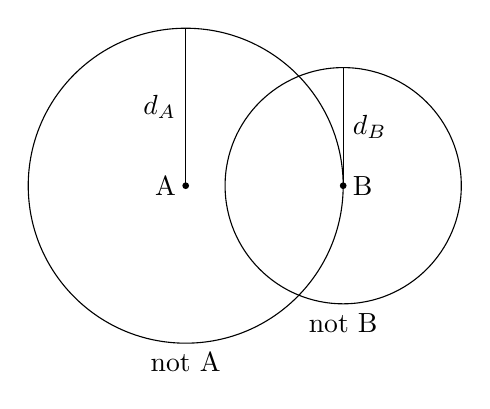
\begin{tikzpicture}
        \coordinate (A) at (0,0);
        \coordinate (Ar) at (0,2);
        \coordinate (Ac) at (0, -2);
        
        \filldraw[black] (A) circle (1pt) node[anchor=east] {A};
        \draw (A) -- node[anchor=east]{$d_A$} ++ (Ar);
        \draw[black] (A) circle (2cm);
        \draw (Ac) node[anchor=north] {not A};
        
        \coordinate (B) at (2,0);
        \coordinate (Br) at (0, 1.5);
        \coordinate (Bc) at (2, -1.5);
        
        \filldraw[black] (B) circle (1pt) node[anchor=west] {B};
        \draw (B) -- node[anchor=west]{$d_B$} ++ (Br);
        \draw[black] (B) circle (1.5cm);
        \draw (Bc) node[anchor=north] {not B};
        
    \end{tikzpicture}
\end{center}

We can now see that there is a circular intersection of the two spheres on which no points are colored $A$ and no points are colored $B$, therefore, this circle must be colored $C$.

\begin{center}
    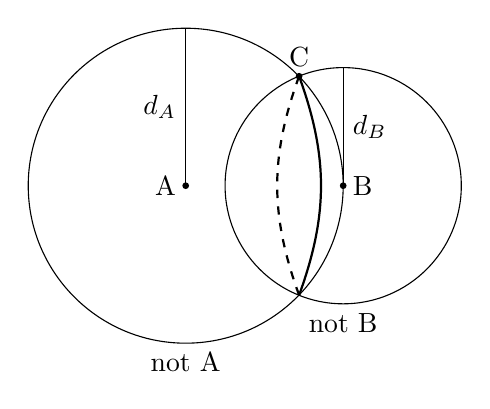
\begin{tikzpicture}
        \coordinate (A) at (0,0);
        \coordinate (Ar) at (0,2);
        \coordinate (Ac) at (0, -2);
        
        \filldraw[black] (A) circle (1pt) node[anchor=east] {A};
        \draw (A) -- node[anchor=east]{$d_A$} ++ (Ar);
        \draw[black] (A) circle (2cm);
        \draw (Ac) node[anchor=north] {not A};
        
        \coordinate (B) at (2,0);
        \coordinate (Br) at (0, 1.5);
        \coordinate (Bc) at (2, -1.5);
        
        \filldraw[black] (B) circle (1pt) node[anchor=west] {B};
        \draw (B) -- node[anchor=west]{$d_B$} ++ (Br);
        \draw[black] (B) circle (1.5cm);
        \draw (Bc) node[anchor=north] {not B};
        
        \coordinate (i1) at (1.44, 1.39);
        \coordinate (i2) at (1.44, -1.39);
        \filldraw[black] (i1) circle (1pt) node[anchor=south] {C};
        \path [thick, black, dashed, out=-110, in=110] (i1) edge (i2);
        \path [thick, black, out=-70, in=70] (i1) edge (i2);
        
    \end{tikzpicture}
\end{center}

To find the radius of this circle, we'll look at this triangle, where $h$ is the radius of our $C$ colored circle.

\begin{center}
    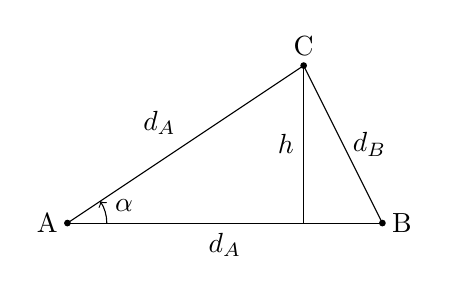
\begin{tikzpicture}
        \coordinate (A) at (0, 0);
        \coordinate (B) at (4, 0);
        \coordinate (C) at (3, 2);
        
        \filldraw[black] (A) circle (1pt) node[anchor=east] {A};
        \filldraw[black] (B) circle (1pt) node[anchor=west] {B};
        \filldraw[black] (C) circle (1pt) node[anchor=south] {C};
        
        \draw (A) -- node[anchor=north]{$d_A$} ++ (B);
        \draw (A) -- node[anchor=south east]{$d_A$} ++ (C);
        \draw (B) -- node[anchor=west]{$d_B$} ++ (-1, 2);
        \draw (3,0) -- node[anchor=east]{$h$} ++ (0,2);
        
        \pic [draw, ->, "$\alpha$", angle eccentricity=1.5] {angle = B--A--C};
        
    \end{tikzpicture}
\end{center}

Using the law of cosines, we can find
\begin{align*}
    \alpha &= \cos^{-1}\left(\frac{d_A^2 + d_A^2 - d_B^2}{2d_Ad_A}\right) \\
    \alpha &= \cos^{-1}\left(\frac{2d_A^2 - d_B^2}{2d_A^2}\right)
\end{align*}
\begin{align*}
    h &= d_A\sin(\alpha) \\
    h &= d_A\sin\left(\cos^{-1}\left(\frac{2d_A^2 - d_B^2}{2d_A^2}\right)\right) \\
    h &= \frac{d_B \sqrt{4 d_A^2 - d_B^2}}{2d_A} \\
    2h &= d_B \frac{\sqrt{4 d_A^2 - d_B^2}}{d_A}  
\end{align*}

If $2h \geq d_B \geq d_C$, then $d_C$ would exist between two points on the circle. $2h \geq d_B$ if
\[\frac{\sqrt{4 d_A^2 - d_B^2}}{d_A} \geq 1\]
which is true if
\[\sqrt{4 d_A^2 - d_B^2} \geq d_A\]
which is true if
\[4 d_A^2 - d_B^2 \geq d_A^2\]
which is true if
\[3 d_A^2 - d_B^2 \geq 0\]
which is true if
\[3 d_A^2 \geq d_B^2\]
and since
\[3 d_A^2 \geq d_A^2 \geq d_B^2\]
we know
\[2h \geq d_c\]
so there is a circle with all points colored $C$ with diameter $2h \geq d_C$ on which $d_C$ must exist between two $C$ colored points.

\begin{center}
    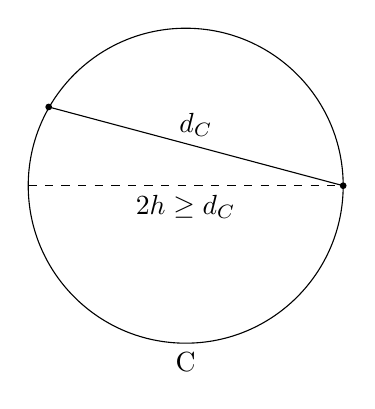
\begin{tikzpicture}
        \draw[black] (0,0) circle (2cm);
        \draw (0,-2) node[anchor=north] {C};
        \draw[dashed] (-2,0) -- node[anchor=north] {$2h \geq d_C$} ++ (4,0);
        
        \filldraw[black] (2, 0) circle (1pt);
        \filldraw[black] (-1.74, 1) circle (1pt);
        \draw[black] (2,0) -- node[anchor=south] {$d_C$} ++ (-3.74,1);
        
        
    \end{tikzpicture}
\end{center}

 Therefore, $d_C \in S(C)$. However this contradicts our earlier statement that $d_C \notin S(C)$. This process can be continued with with any set of $\{d_A \notin S(A), d_B \notin S(B), d_C \notin S(C)\}$ until all distances in one of the colors can be shown to exist in our colored space. Thus, our assumption cannot be true. So at least one color in our space must attain all distances.


\newpage
\section*{Problem 9}
\fbox{
    \parbox{\textwidth}{
        Show that the interval [0,1] cannot be partitioned into two disjoint sets $A$ and $B$ such that $B = A + a$ for some real number $a$.
    }
}
\\

We will first assume that it is possible to partition the interval $S = [0, 1]$ into two disjoint sets $A$ and $B$ such that $B = A + a$ for some real number $a$. Since $S$ is being partitioned into $A$ and $B$,
\begin{equation} \label{part}
    (A \cup B) = S = [0,1]
\end{equation}
\begin{align}
    A \subset S \label{asub} \\
    B \subset S \label{bsub}
\end{align}
Since $A$ and $B$ are disjoint sets,
\begin{equation} \label{disj}
    (A \cap B) = \varnothing
\end{equation}
Since
\begin{equation} \label{func}
    B = A + a
\end{equation} for some real number $a$. We also know that
\begin{align}
    A \ne \varnothing \label{afull} \\
    B \ne \varnothing \label{bfull}
\end{align}
since if either $A$ or $B$ were the empty set, \eqref{func} would tell us that both are the empty set. Which would make \eqref{part}
\[[0,1] = S = (A \cup B) = (\varnothing \cup \varnothing) = \varnothing\]
but
\[[0,1] \ne \varnothing\]
which is a contradiction, therefore \eqref{afull} and \eqref{bfull} must be true.

To show why $a \ne 0$, we will first assume that $a=0$. This would mean that \eqref{func} would become
\begin{equation} \tag{\ref{func}$^\prime$} \label{func-prime}
    B = A
\end{equation}
Taking \eqref{disj} and substituting with \eqref{func-prime}, we get
\[(A \cap A) = \varnothing\]
and since the intersection of a set and itself is itself, we get
\[A = \varnothing\]
This,  with \eqref{afull}, is a contradiction, so our assumption that $a=0$ is false, therefore $a \ne 0$. 

We will also consider $a$ to be a positive value, and $A$ and $B$ to be the sets which satisfy \eqref{func} for a positive $a$ value. If $a$ were negative, we would just swap $A$ and $B$ in all instances, since it only matters that they are distinct sets. So $a > 0$. 

\begin{framed}
    To show $0 \in A$.
    \begin{enumerate}
        \item Assume $0 \notin A$.
        \item $0 \in B$ from \eqref{part} and step 1.
        \item Some negative number $-a \in A$ from \eqref{func} on step 2.
        \item Some negative number $-a \in S$ from \eqref{asub} on step 3.
        \item However, $S = [0,1]$ contains no negative numbers.
    \end{enumerate}
    Steps 5 and 6 are a contradiction, therefore our assumption is false, so $0 \in A$. 
\end{framed}

And by \eqref{func}, we know that $a \in B$. And by \eqref{asub} and \eqref{bsub}, we know
\begin{equation} \label{0aS}
    [0,a] \subseteq S
\end{equation}

\begin{framed}
    To show $[0, a) \subseteq A$.
    \begin{enumerate}
        \item Assume $[0, a) \not \subseteq A$.
        \item $\exists (c \in S)[0 < c < a, c \in B]$ from \eqref{0aS} and step 1
        \item $(c-a) \in A$ from \eqref{func} on step 2.
        \item $(c-a) \in S$ from \eqref{asub} on step 3.
        \item $(c-a)$ is negative since $c < a$ from step 2.
        \item However, $S = [0,1]$ contains no negative numbers.
    \end{enumerate}
    Steps 4, 5, and 6 are a contradiction, therefore our assumption is false, so 
\end{framed}
\begin{equation} \label{0aA}
    [0, a) \subseteq A
\end{equation}
and from \eqref{func} and \eqref{0aA}, we know
\begin{equation} \label{a2aB}
    [a, 2a) \subseteq B
\end{equation}

We will take \eqref{0aA} and \eqref{a2aB} as our base case for induction. 

\newpage
\begin{framed}
    For our inductive step, we will assume we know that for some $n \in \mathbb{N}$
    \[A_n = na, (n+1)a) \subseteq A\]
    \[B_n = [(n+1)a, (n+2)a) \subseteq B\]
    \begin{enumerate}
        \item $(n+2)a \in S$ since $B_n$ is open on the right, $S$ is closed in the right, and $B_n \subset S$.
        \begin{framed}
            To show $(n+2)a \in A$
            \begin{enumerate}
                \item Assume $(n+2)a \notin A$
                \item $(n+2)a \in B$ from \eqref{part} and step 1 and step a.
                \item $(n+1)a \in A$ from \eqref{func} and step b.
                \item $(n+1)a \in B$ from given definition of $B_n$.
                \item $(n+1)a \in A \cap B$ from definition of set intersection, step c, and step d.
                \item $(n+1)a \in \varnothing$ from substitution on \eqref{disj} and step e.
            \end{enumerate}
            Step f is a contradiction, therefore our assumption is false so
        \end{framed}
        \item $(n+2)a \in A$.
        \item $(n+3)a \in B$ from \eqref{func} on step 2.
        \begin{framed}
            To show $[(n+2)a, (n+3)) \subseteq A$.
            \begin{enumerate}
                \item Assume $[(n+2)a, (n+3)) \not \subseteq A$.
                \item $\exists (c \in S)[(n+2)a < c < (n+3)a, c \in B]$ from \eqref{0aS} and step a
                \item $(c-a) \in A$ from \eqref{func} on step b.
                \item $(n+1)a < (c-a) < (n+2)a$ from step b and step c.
                \item $(c-a) \in [(n+1)a, (n+2)a) = B_n$ from given definition of $B_n$.
                \item $(c-a) \in B$ from definition of $B_n$, definition of a subset, and step e.
                \item $(c-a) \in A \cap B$ from definition of set intersection, step c, and step f.
                \item $(n+1)a \in \varnothing$ from substitution on \eqref{disj} and step g.
            \end{enumerate}
            Step h is a contradiction, therefore our assumption is false, so 
        \end{framed}
        \item $[(n+2)a, (n+3)a) \subseteq A$.
        \item $[(n+3)a, (n+4)a) \subseteq B$ from \eqref{func} and step 4.
    \end{enumerate}
    
\end{framed}

Since $A_0 \subseteq A$ and $B_0 \subseteq B$ from \eqref{0aA} and \eqref{a2aB}, respectively, we can show that for any $n \in \mathbb{N}$, we can get $na, (n+1)a) \subseteq A$, which means $na \in A$, which means $na \in S$. This means that if we make
\begin{align*}
    n &> \frac{1}{a} \\
    na &> 1 \\
\end{align*}
we can show some number $na > 1$ and $na \in S$. However, $S=[0,1]$ has no elements greater than 1. So this is a contradiction, therefore, our assumption must be false, so the interval [0,1] cannot be partitioned into two disjoint sets $A$ and $B$ such that $B = A + a$ for some real number $a$.

\end{document}